% File: tex/methods.tex
% Author: Timo L. R. Halbesma <timo.halbesma@student.uva.nl>
% Version: 0.01 (Initial)
% Date created: Sat Oct 24, 2015 12:28 am
% Last modified: Mon Sep 05, 2016 02:28 PM
%
% Description: Masterthesis, Methods


\documentclass[MScProj_TLRH_ClusterEnergy.tex]{subfiles}
\begin{document}
\chapter{Methods}
\label{sec:methods}

Numerical simulations provide a great tool to gain insight into the realm of
astronomy otherwise unaccessible in studies that require tweaking of the system
parameters. In our case, we are interested in the impact that a major merger has
on the intra cluster medium surrounding Cygnus~A. It is impossible to study this 
phenomenon in a laboratory, and the timescales involved are millions of years so
we are unable to just wait around until something has changed significantly. This 
object is an excellent candidate to study by running a grid of simulations 
with different underlying model parameters. Our numerical representations of the
CygA and CygB can bridge the gap between theory and observations. At present, 
the simulation pipeline is threefold. First, we set up initial conditions that
allow us to tweak the model parameters of both haloes. An explanation of how we
infer some hard constrains on the initial conditions from the X-ray observations 
can be found in chapter~\ref{sec:constrains}, and the way these constants propagate
trough in the numerical setup is presented in section~\ref{sec:methods-toycluster}.
Secondly, a file that contains the sampled particles is passed to a combined 
gravity-hydro solver as described in section~\ref{sec:methods-gadget}.
Finally, the three-dimensional simulation snapshots are integrated along a 
chosen line of sight and observables such as the X-ray surface brightness and 
the spectroscopic temperature are calculated. Details of this last step are given 
in section~\ref{sec:methods-psmac}. As the underlying hydro method is Smoothed
Particle Hydrodynamics (SPH), we first cover the basics in 
section~\ref{sec:methods-hydro}.

% \section{Gravitational Solvers}
% \label{sec:methods-gravity}
% 
% \section*{A hierarchical O(N log N) force-calculation algorithm}
% \label{sec:BarnesHut1986}
% Summary of \citet{1986Natur.324..446B}.
% \\
% A new method has been developed to calculate the gravitational force directly at cost of $N \log N$, instead of the direct integration method which is accurate but computationally expensive ($N^2$). The authors split space up in cubic cells at every time step to generate an oct-tree by using a recursive algorithm terminating once all cells contain one particle only. The Barnes-Hut method replaces i) direct integration and ii) a potential fitting method which tracks particle movement trough the potential field and is of order $N \log N$, albeit at significantly lower accuracy and with loss of generality. Generality is lost because the specific implementation (Fourier, spherical or bispherical harmonics) requires a specific geometry.
% 
% Other methods are considered as well, but their disadvantages are emphasised (difficult to analyse the significant accumulation of errors) as a result of improved cost. Here, on the other hand, it is possible to directly calculate the forces as $N \log N$ by hierarchically (ab initio at every time step) grouping space in cubical cells, splitting up cells to half the length if the cell until all cells contain one particle. Then discard empty cells. Higher-order cells with multiple particles are represented by a pseudo-particle at the center of mass with the total mass of the cells. Lumping together particles is done based on the `opening angle' criterion. This procedure yields a cost of the height of the tree $O(\log_2 N^{1/3})$ for force calculations, and tree construction is $O(N \log N)$. The next step is tagging subdivided cells with total mass and center-of-mass positions, which is also $O(N \log N)$.
% 
% The force is calculated if the opening angle criterion is met. The tree is traversed from the root downwards. Whether the force acting on a particle $p$ from the `active' tree cell is calculated if $l/D < \theta$, where $l$ is the length of the cell, $D$ is the distance from $p$ to the center of mass of the cube considered. The opening angle criterion $\theta$ acts as the (fixed) accuracy parameter and is chosen unity here. If the criterion is not met, the procedure is recursively continued on the eight subcells. In this case the number of calculations is a function of $\theta$, not $N$, thus $\log N$ computations are required % the last sentence is probably not fully correctly paraphrased here...
% 
% It is possible to do a rigorous error analysis on this newly proposed method. If a cell is chosen not to be subdivided (due to opening angle), then the error is accumulated because of the quadrupole and higher order moments that are neglected in approximating the force. Most importantly, the errors are weakly correlated between times steps resulting in error accumulation reminiscent of a random walk instead of systematic error build up.
% 
% Finally, ways to improve the code and a justification of the implementation in C over FORTRAN is presented by the authors.
% 
% 
% 
% \section{Model setup}
% TODO: this is probably best in a new section since this is not really the method but it is not results yet.
% 
% TODO: write something about test simulations run? Like the Sod Shock tube \citep{1978JCoPh..27....1S}.
% 
% TODO: describe initial and boundary conditions.
% 
% TODO: write about model setup. Obtain parameters and such from the physics of the merger of Cygnus A found in \citep{1999ApJ...521..526M}.
% 
% TODO: write about previously run simulations, like the `off-axis cluster mergers' paper \citep{2001ApJ...561..621R}, and look at the merger simulation of the A754 cluster of galaxies \citep{1998ApJ...493...62R}.
% 
% Relevant for initial conditions? "We have spectroscopically identified 77 new
% members of the Cygnus A cluster, bringing to 118 the total number of galaxies
% consistent with cluster membership ... The data are consistent with a
% cluster-cluster merger viewed at a projection angle of $30^\circ-40^\circ$,
% $0.2-0.6$ Gyr prior to core passage ... Markevitch et al. (1999) estimate a
% subcluster collision velocity of $2200^{+700}_{-500}$ km s$^{-1}$. ...  Within a
% 500 kpc radius, Smith et al. (2002) derive a gas mass of 1.1 $\times 10^{13}$
% M\Sun and a total mass between $(2.0 - 2.8) \times 10^{14}$ M\Sun (depending on
% the central temperature profile). We estimate a factor of 4–5 higher total mass,
% based on the projected mass from the optical data. However, it is difficult to
% compare both." \citep{2005AJ....130...47L}.
% 
% TODO: add iPython notebook comments for initial conditions
% 
% 
% TODO: 
% 
% We are interested in solving the equations of motions in three dimensions for a
% finite number of particles $N$. The most intuitive way to solve the
% gravitational component is to calculate Newton's law of gravity plus the
% contribution of an external potential field. A computational problem occurs when
% the distance between two particles decreases ($r\rightarrow$0) resulting in the
% force-term increasing to arbitrary large numbers.
% 
% % This could be overcome by implementing an adaptive timestep that decreases in
% % order to track close encounters of particles at cost of lowering the overall
% % timestep for all particles. This results in extremely long calculations while
% % only one two of the particles are in conflict.
% 
% For this reason the distance between two nearby particles is often softened by
% $\epsilon$, thus, $r \rightarrow r+\epsilon$. Regarding the number of
% calculations, every particle feels the force of all other particles so for every
% particle the force of all other particles acting on it must be calculated. This
% is called the direct $N$-body method for which the resulting computational cost
% is $N(N-1) \rightarrow O(N^2)$, which scales very poorly for increasing $N$. On
% the other hand, apart from the softened close encounters, this methods does
% yield highly accurate results since no further approximations have to be made.
% But cosmological simulations call for the need of very high $N$ and the usage of
% computational facilities is costly. Therefore speed-up is desired albeit at cost
% of accuracy.
% 
% TODO: Direct N-body vs. Tree
% 
% TODO: Hierarchical tree algorithms (Appel 1985, \citep{1986Natur.324..446B}, Dehnen 2000) have no intrinsic resolution limit, but are substantially slower than Fourier-based methods. See p1106 of Springel 2005.
% 
% TODO: Particle-mesh (PM) (e.g. Klypin \& Shandarin 1983; White, Frenk \& Davis
% 1983; \citep{1988csup.book.....H}) are fast, but on scales smaller than one or
% two mesh cells the force is suppressed which leads to very poor spatial
% resolution. Resolution can be improved (short-range direct-summation forces,
% adding additional Fourier meshes adaptively placed on interesting regions, using
% relaxation methods to adaptively refine the mesh). See p1106 of Springel 2005.
% 
% 
% TODO: TreePM hybrid methods (\citep{1995ApJS...98..355X}) combines both by
% long-range PM and short-range Tree algorithms. See p1106 of Springel 2005.
% Winning? According to Wikipedia it is absolute though. Maybe not winning?


\section{Numerical Hydrodynamics}
\label{sec:methods-hydro}

Smoothed Particle Hydrodynamics (SPH) and Adaptive Mesh Refinement (AMR) are the
two main methods widely used for numerical hydrodynamics. The former is a scheme 
based on the discretization of mass, whereas the latter is a discretization of 
space. SPH is the Lagriangian approach where tracer particles are moving along
with the flow of fluids, while fluid elements placed on a grid in AMR is the 
Eulerian implementation. A schematic representation of a (fixed) grid and SPH is 
shown in Figure~\ref{fig:amr_vs_sph}. Both methods come with their own advantages and 
disadvantages. One of the main strengths of AMR is that shocks are very accurately
treated, especially in comparison to SPH where numerical viscosity inevitably 
smears out the shocks. On the other hand, AMR has discontinuities between every grid 
cell by design. Moreover, cosmological codes require an enormous dynamical range
as the densities involved span several decades, which SPH handles really well. 
Regions of high density can easily be represented by additional particles, 
while lower-density regions are represented by less particles. Merging clusters 
of galaxies will displace the fluid particles along with the merger such that
the method naturally places more particles in the region of interest. Implementing 
our own hydro code is way beyond the scope of a master's project and selecting
either AMR of SPH is beyond our control. We make us of the publicly available
code \code{Gadget-2}, which implements SPH. Therefore we briefly discuss the
basics of SPH in order to understand the simulations to assess the validity and
trustworthiness of the output.

\begin{figure}
    \centering
    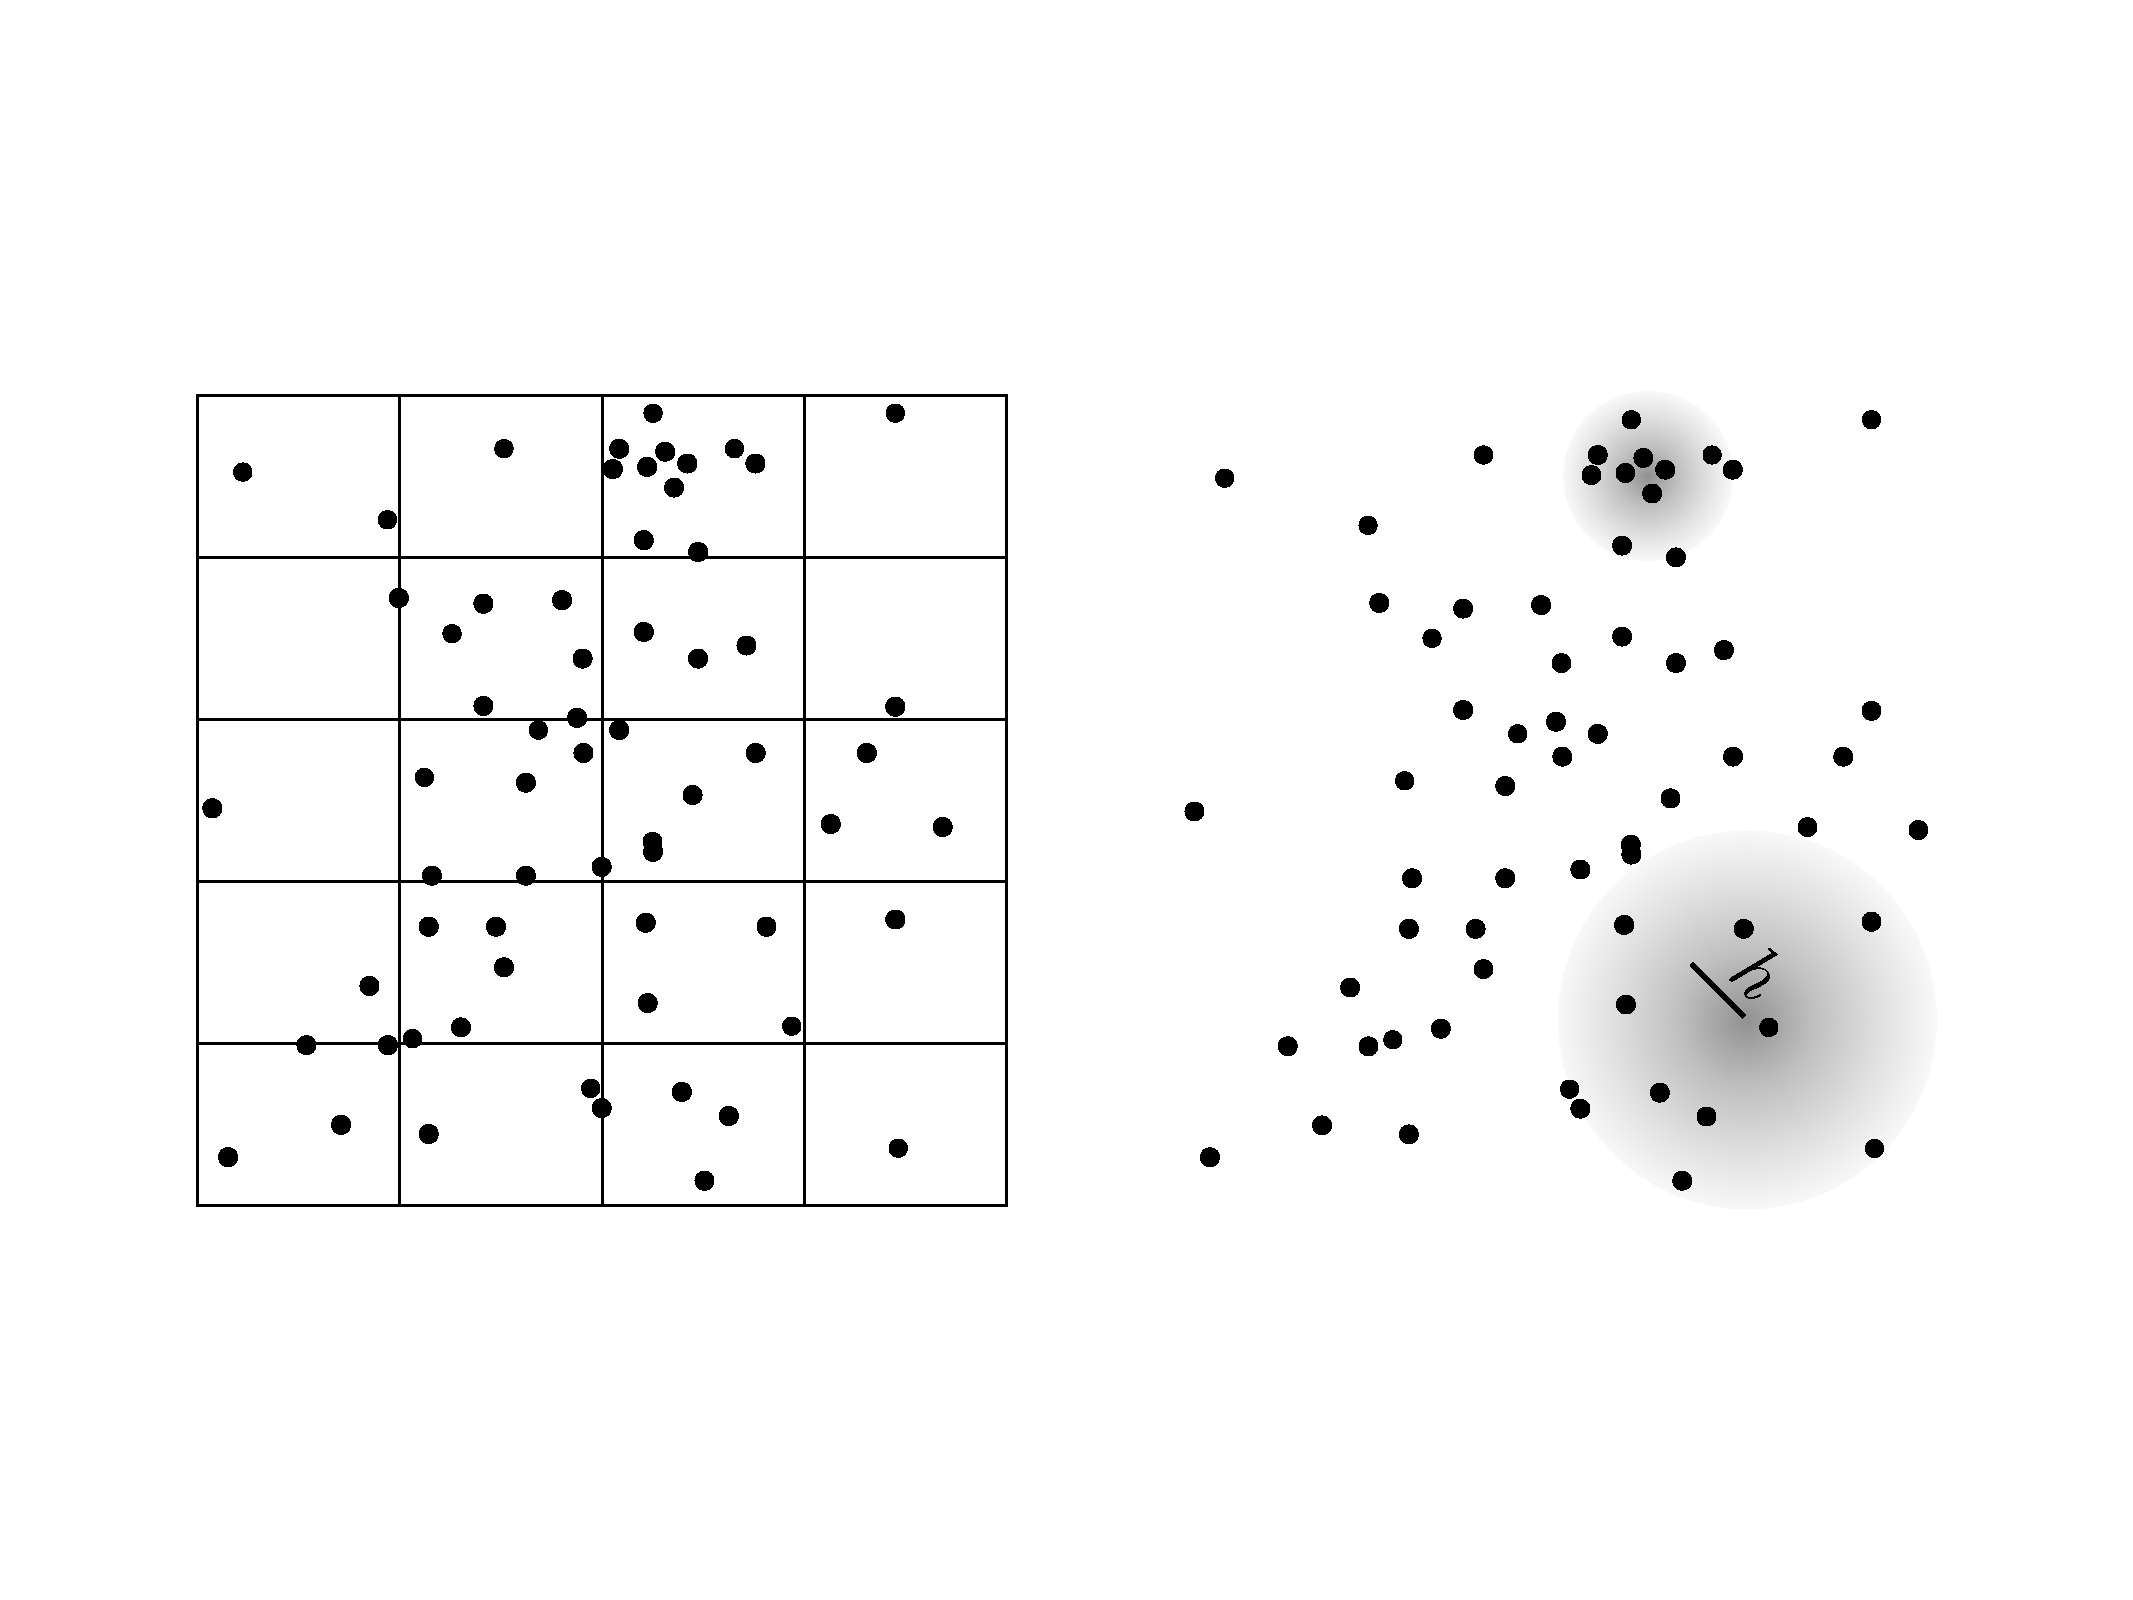
\includegraphics[width=0.78\textwidth]{methods/sph.pdf}
    \caption{\textbf{Left:} Particles on a (fixed) grid. \textbf{Right:} SPH 
             particles follow fluids and smooth over particles within
             two (kernel-dependent) times the smoothing radius $h$. Image reproduced from 
             \citet{Price2012759}.}
    \label{fig:amr_vs_sph}
\end{figure}


The mathematical framework for SPH was simultaneously formulated by 
\citet{1977AJ.....82.1013L} and \citet{1977MNRAS.181..375G}, and a more recent
pedagogical review of SPH in an astrophysical context is published by
\citet{Price2012759}. An accurate calculation of the density is the most important 
in SPH as all other physical quantities are derived from it. The method represents
fluids as particles where the density of particle $j$ is calculated by weighted 
summation over nearby single-particle densities for NGB number of neighbours.
The weight given depends on the distance and is described by a mathematical 
weighing function $W$ called the smoothing kernel. \citet{Price2012759} gives 
the requirement that SPH-kernels must
\begin{enumerate}[i)]
    \item have a flat top in the center because otherwise the density estimate
          would be severely influenced when the position of nearing neigbhours
          changes;
    \item converge to a finite value, or be truncated at certain radius;
    \item have smooth derivatives and decrease monotonically with relative distance;
    \item show symmetry such that $W(\mathbf{r}'-\mathbf{r},h) \equiv 
          W(|\mathbf{r}-\mathbf{r'}|,h)$.
\end{enumerate}

\noindent The density $\rho$ is then given by
\begin{align}
    \rho (\mathbf{r}) &= \sum\limits_{b=1}^{\text{NGB}} m_b
        W(\mathbf{r}-\mathbf{r_b}, h) \label{eq:sphdensity} \quad ,
\end{align}
\noindent where $h$ is a scale parameter that sets the fall-off rate of the
smoothing kernel as a function of particle spacing.

The most straightforward implementation is the Gaussian. Adopting this kernel, 
however, in principle requires smoothing over all particles because the function 
does not converge at a finite radius. Moreover, particles further away weigh 
significantly less than nearby particles which means a lot of computational time
is spent calculating relatively unimportant contributions. A full discussion of
the implementation and nuances of SPH is beyond the scope of this thesis, but we 
briefly discuss two alternatives. The alternatives behave like the Gaussian
but converge at a given radius, a concept called compact support. While
this does result in a less accurate density estimate that is more sensitive
to changes in nearby particles, the computational cost 
scales much more favourably as $O(N \cdot NGB)$ for $N$ particles instead of 
$O(N^2)$ when using the Gaussian. Initially, SPH implementations used the 
\citet{SchoenbergBSpline} B-spline functions 
\citep{1985JCoPh..60..253M, 1985A&A...149..135M}, which not surprisingly,
is adopted in \code{Gadget-2}. State of the art SPH implementations
nowadays, however, use \citet{wendland1995piecewise, wendland2004scattered} 
polynomials for better accuracy and less instability \citep{2012MNRAS.425.1068D}.
For this reason, \code{Toycluster} uses the Wendland~C6 kernel rather than the 
older B-spline. Figure~\ref{fig:kernels} show these three functions, where 
$w(q=r/h) = h^3 W(|\mathbf{r}-\mathbf{r_b}|, h)$ in three dimensions.
The subplot on the left shows the functions for $h=1$ on the domain $q \in [0, 3]$,
while the values are divided over their own normalisation factor in the panel 
on the right to place them the same scale, and the y-axis is logarithmic. This 
clearly shows that both the cubic spline and the Wendland~C6 polynomial converge 
at $q=2$, while the Gaussian does not converge and is truncated at $r=3$.

\begin{figure}[ht]
  \centering
  \begin{subfigure}[b]{0.5\textwidth}
    \centering
    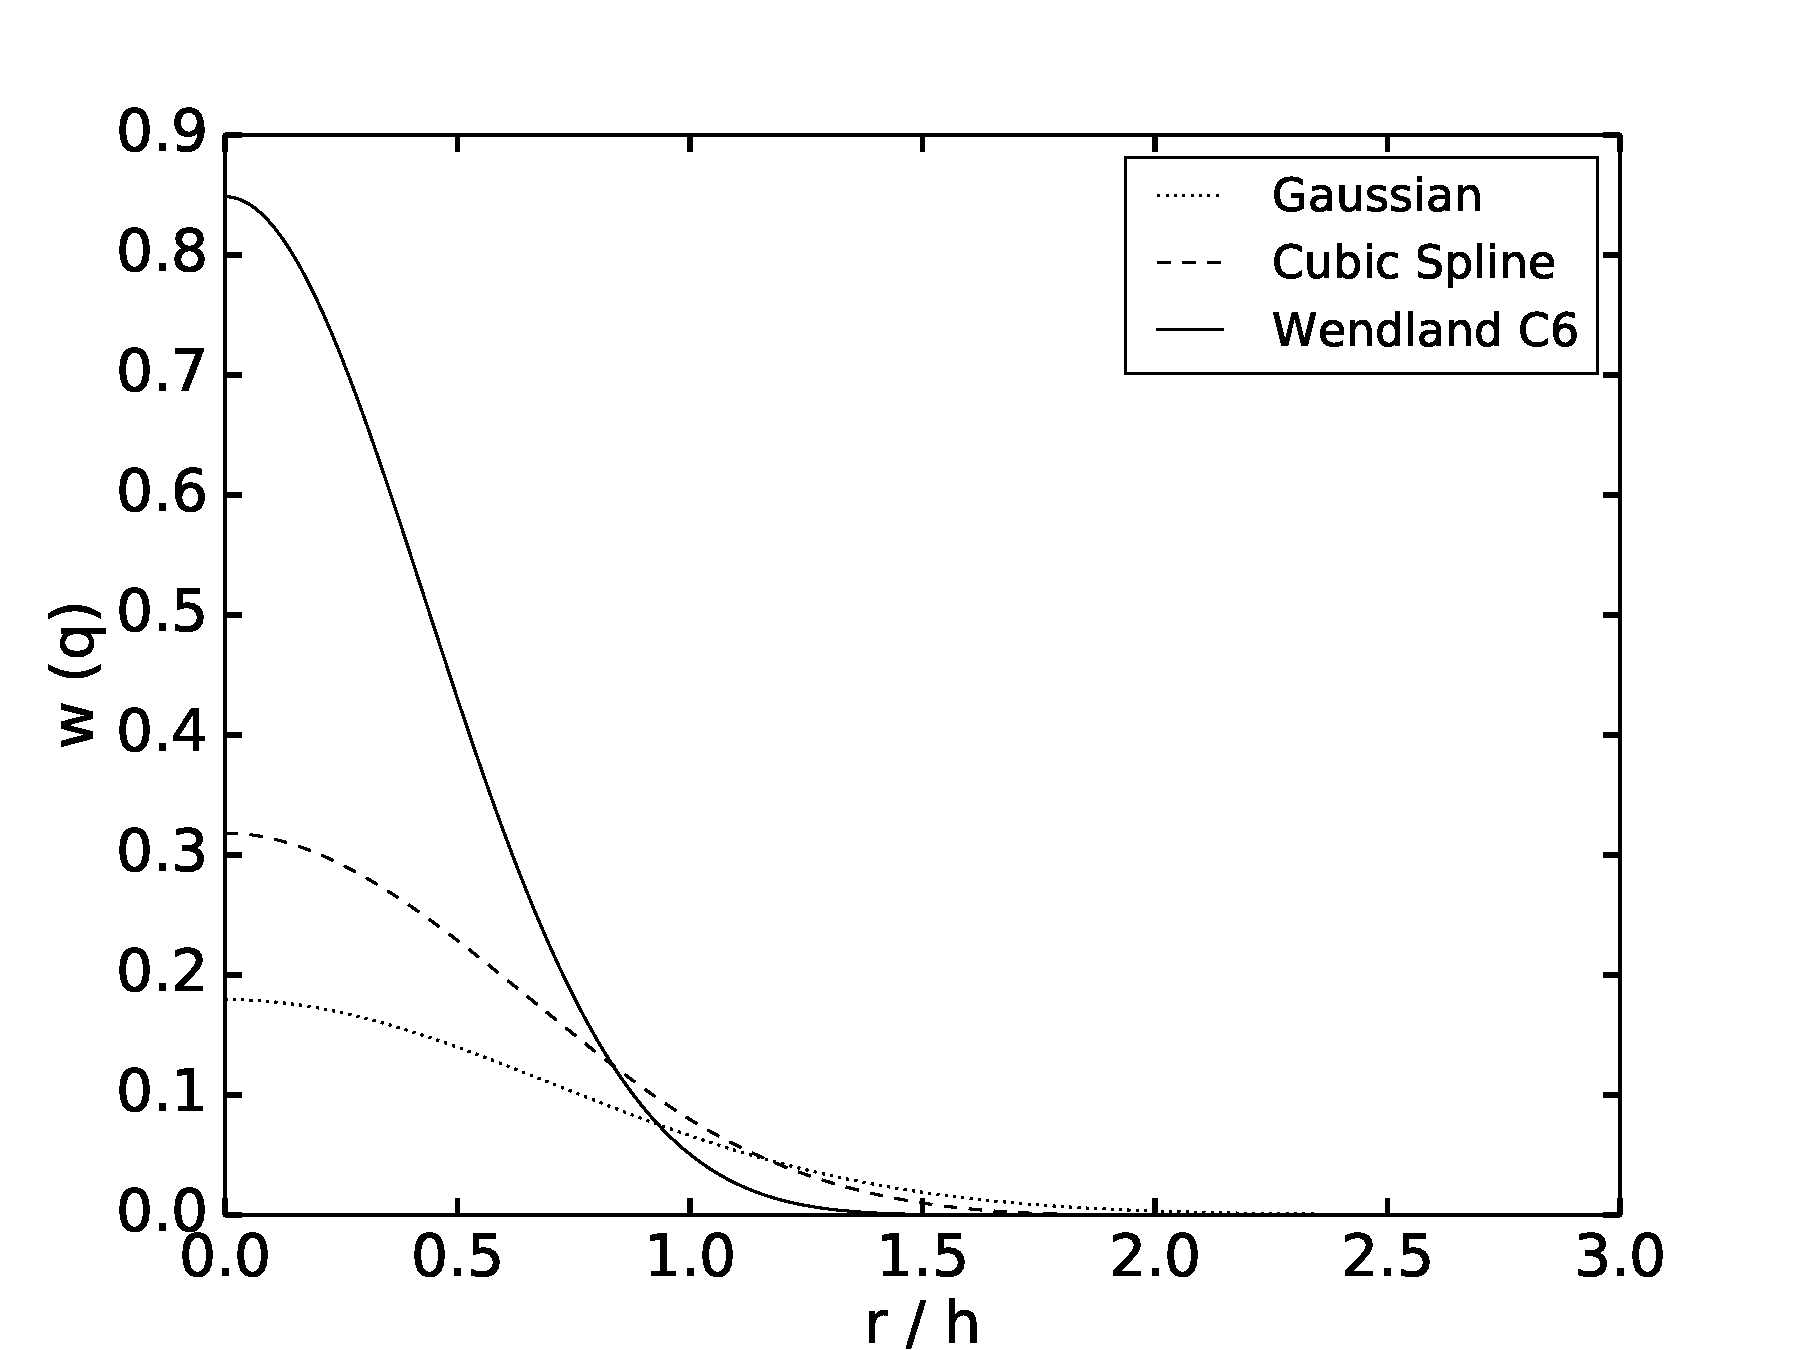
\includegraphics[width=\linewidth]{methods/kernels/kernels.pdf}
  \end{subfigure}%
  ~
  \begin{subfigure}[b]{0.5\textwidth}
    \centering
    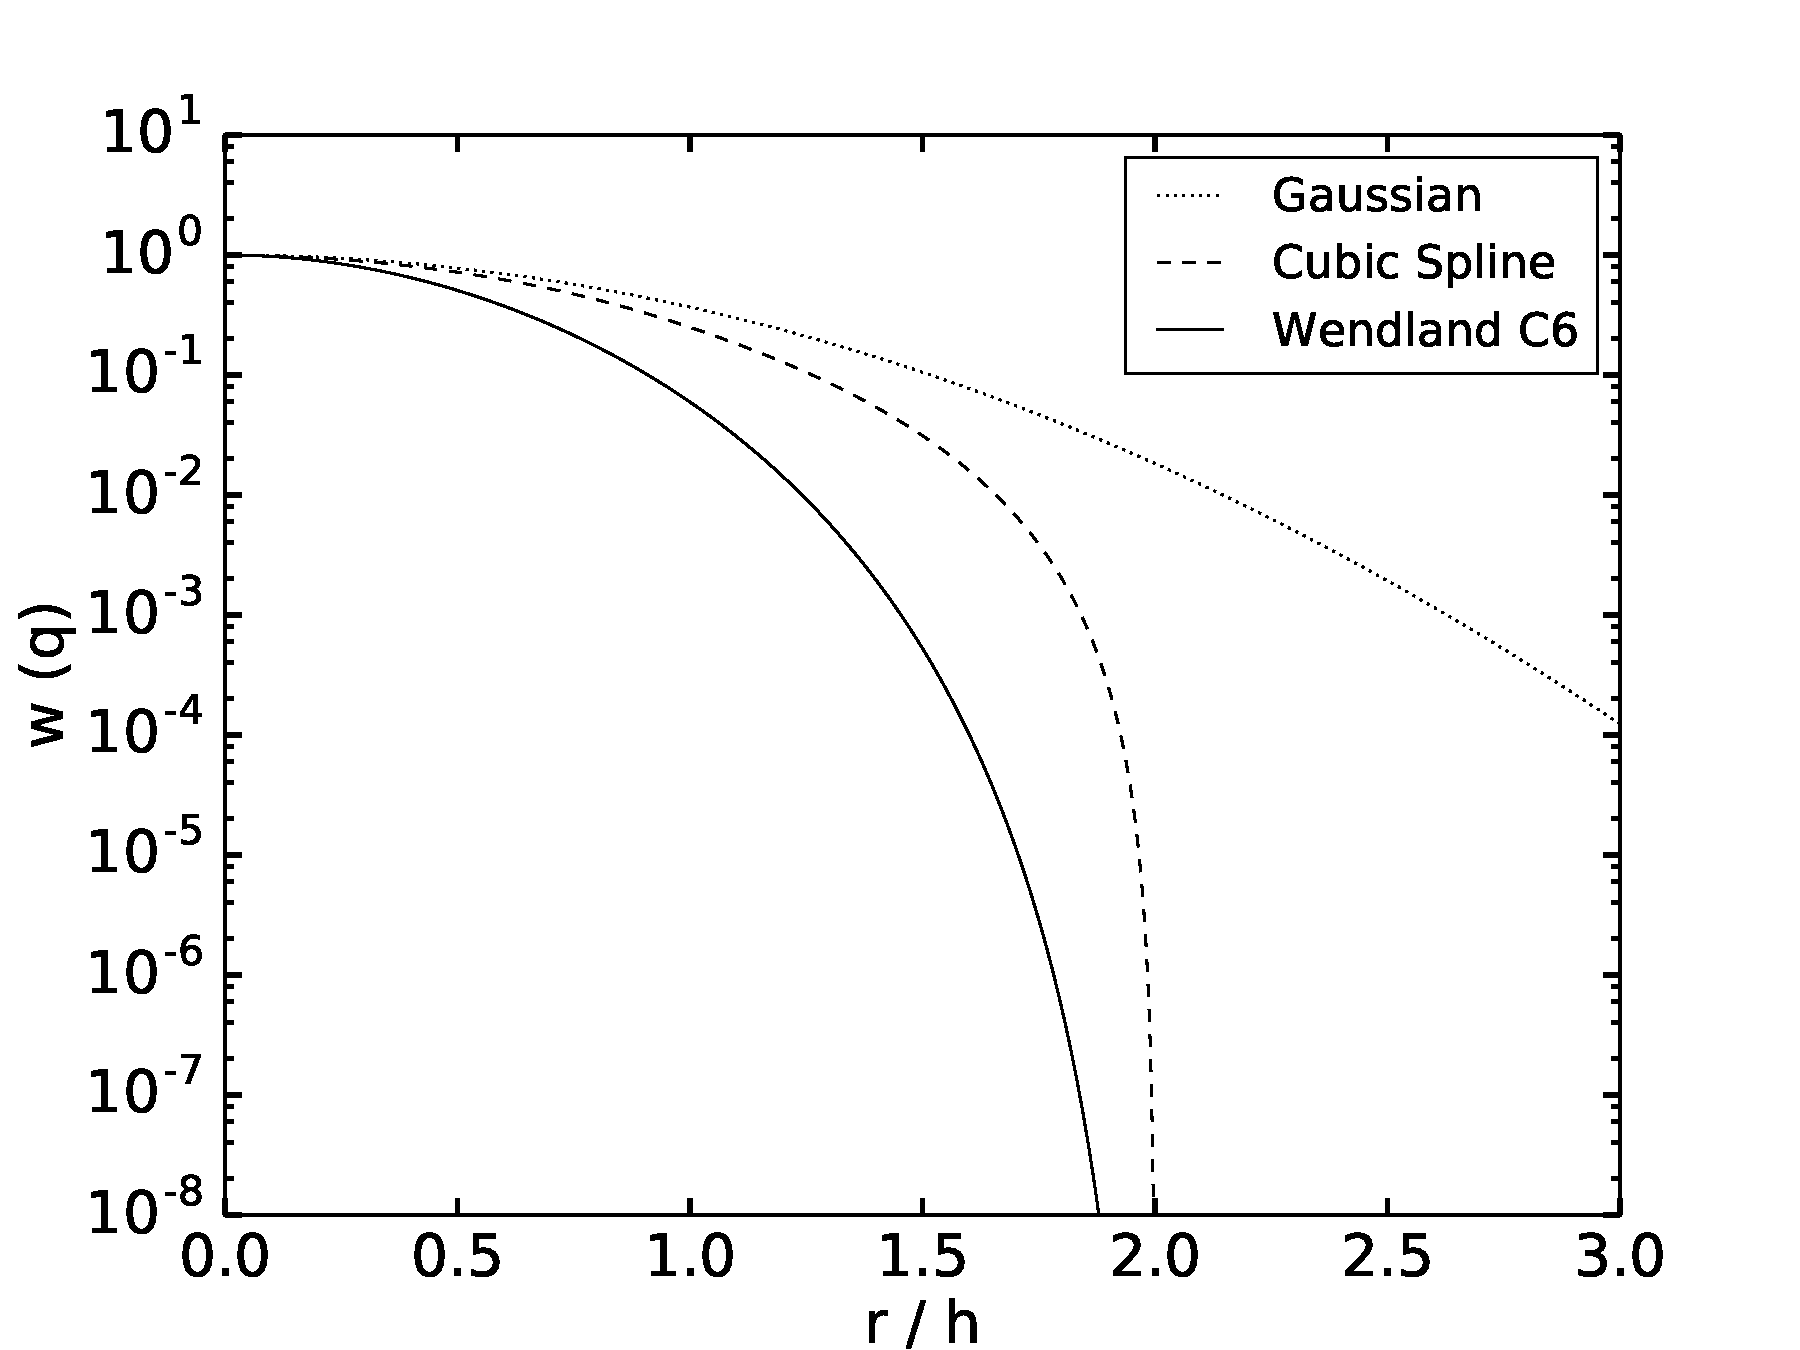
\includegraphics[width=\textwidth]{methods/kernels/kernels_logy_normalised.pdf}
    \end{subfigure}
    \caption{\textbf{Left}: Gaussian, \citet{SchoenbergBSpline} Cubic B-Spline~(M4),
             and \citet{wendland1995piecewise}~C6 kernels.
             \newline
             \textbf{Right:} Same kernels, but normalised and shown on a logarithmic
             scale. The Gaussian is truncated at $r=3h$ while the other two kernels
             have compact support at $q=r/h=2$.}
    \label{fig:kernels}
\end{figure}

The generalisation of hydrodynamic quantities in SPH is as follows
\begin{align}
    A(\mathbf{r}) &= \sum\limits_{j} m_j \frac{A_j}{\rho_j}
        W(|\mathbf{r}-\mathbf{r_j}|,h) \label{eq:sph} \\
    \nabla A(\mathbf{r}) &= \sum\limits_{j} m_j \frac{A_j}{\rho_j} 
        \nabla W(|\mathbf{r}-\mathbf{r_j}|,h)
        \label{eq:sphderivative} \quad ,
\end{align}
\noindent where $A(r)$ is the quantity of interest, $m_j$ the mass of particle
$j$, $A_j$ its finite value, $\rho_j$ the density, and $W$ is the kernel function.
The beauty of these equations is that all particle values are constants such that
the derivative $\nabla A(r)$ is then obtained by deriving the kernel, which is
why the third kernel requirement is that the function has smooth derivatives.

TODO: hsml finding.





\section{\code{Toycluster}: Stable Initial Conditions}
\label{sec:methods-toycluster}
The initial conditions generating code was not written by the author of this
thesis. We make make use of the proprietary code \code{Toycluster} written by 
\citet{2014MNRAS.438.1971D}. In the time since this publication, changes to the
code have been made that will soon be published by \citet[in prep]{2016MNRAS.000.000D}.
In this section we summarise the numerical setup and highlight changes in the 
latest version with respect to the 2014 (legacy) version.

There are two main approaches when simulating merging clusters of galaxies. On the
one hand, one can simulate the dark-matter dominated large-scale structure of 
the universe (\ref{sec:structure}) in cosmological gravity-only simulations.
The baryonic content can then be added later on to a region of interest. Such 
simulations naturally take into account the substructure of dark matter haloes 
and their movement along the cosmic filament. While such an approach does result in more 
accurate simulations, the down side is that the majority of the computational time
is spent tracking large regions irrelevant to the cluster-cluster merger. 
Moreover, mergers in such simulations are more rare events, and finding one that 
matches the observations of the desired cluster is even more difficult. On the 
other hand, these issues are solved naturally in the second approach, where one 
simulates isolated binary cluster mergers. This allows to tweak both haloes 
involved as well as the kinematics of the merger by altering the parameters when
sampling the individual clusters and placing them on the desired collision course.
Although this is computationally much more favourable, the downside is that this 
type of simulation is (highly) idealised and is therefore less realistic because
the actual physical processes are more complicated than assumed. Furthermore, a
requirement for binary mergers is that the system involved can be approximated
by the hydrostatic equation. When discussing the desired method for the Cygnus~A
cluster, we point out that the mosaic in Figure~\ref{fig:CygA_Xray_extended} 
shows X-ray emission that seems fairly relaxed, indicating that the cluster has 
not likely undergone significant interactions over the dynamical timescale and,
consequently, can be considered in hydrostatic equilibrium. This particular system
is thus deemed suitable to simulate as a binary merger. Again, choosing one of
both is out of our hands as the code is not self-written by the author of this
thesis.

% It is essential to adopt the latest and most accurate cosmological parameters 
% for high-precision cosmology studies. We, on the other hand, choose to adopt 
% concordance cosmology
% It is not our intention to 
% perform high-precision cosmological simulations, the statistical errors of
% our observations fall within the thirty to forty per cent regime while 
% systematic biases dominate the uncertainty of this study such that we would not 
% benefit from more accurate cosmological parameters, or experience severe errors 
% in our analysis as a result of the specific cosmological values chosen. The 
% effect of adopting generic cosmological parameters would be at the per cent 
% level, at best. 
% % ------------------------------------------------------------------------
% 
% 
% 
% 
% 
% 
% 
% 
% 
% 



\section*{Additional Cut-off in Betamodel}

In \code{Toycluster}, merging clusters of galaxies are set up as idealised binary
mergers in a box with periodic boundary conditions. The intra cluster medium is
assumed to be in hydrostatic equilibrium, and the haloes are spherically symmetric.
The hydrostatic equation is solved analytically in the legacy version, while newly
implemented physical models require a numerical approach. The system is set up 
for Smoothed Particle Hydrodynamics, and the dark matter content is implemented
by means of collisionless particles that will interact gravitationally but are 
not considered by the hydrodynamics. The models further ignore star formation, 
supernova enrichment of the hot intra cluster medium, AGN-feedback, galaxies,
and the intra cluster light. The dark matter haloes follow the
\citet{1990ApJ...356..359H} density profile, equation~\eqref{eq:hernquist} in
section~\ref{sec:darkmatter}, and the gas is set up with the beta-model 
\citep{1978A&A....70..677C}, equation~\eqref{eq:betamodel} in 
section~\ref{sec:clustergas}. \citet{2014MNRAS.438.1971D} assumes a fixed value
of $\beta = 2/3$ \citep{2008MNRAS.389..967M}, which results in an analytical 
expression for the mass, gravitational potential, and the hydrostatic equation.
The gas density profile is slightly modified in the latest version of the code 
as the betamodel is multiplied by an additional factor to enforce a cut-off
at the virial radius. This purely numerical feature is found by trial-and-error
to significantly increase the long-term stability of the sampled haloes. The 
reason for the enhanced stability is that the cut-off results in a gas density 
that remains below the dark matter density such that the local baryon fraction
is below unity everywhere in the simulation box \citep[in prep]{2016MNRAS.000.000D}.
The resulting analytical $\beta = 2/3$ expressions with cut-off adopted from 
the aforementioned reference are as follows.
\begin{align}
    \rho_{\text{gas}} (r) &= \rho_0
        \left( 1 + \frac{r^2}{r_c^2} \right)^{-\frac{3}{2}\beta} \cdot
        \left( 1 + \frac{r^4}{r_{\text{cut}}^4} \right)^{-1} \label{eq:betamodel_cut}  \\
    M(<r) &= \frac{4 \pi \rho_0 r_c^2 r_{\text{cut}}^3}{8( r_{\text{cut}}^4+r_c^4)} \cdot \Bigg[ - 8  r_c  r_{\text{cut}}  \arctan(r/rc) + \nonumber \\
&\phantom{{}={}} \sqrt{2} \bigg( (r_c^2-r_{\text{cut}}^2) \Big( \log(r_{\text{cut}}^2 - \sqrt{2}r_{\text{cut}}r+r^2) 
- \log(r_{\text{cut}}^2 + \sqrt{2}r_{\text{cut}}r+r^2)\Big) \nonumber \\
&- 2  (r_c^2 + r_{\text{cut}}^2)  \arctan(1 - \sqrt{2}r/r_{\text{cut}}) 
+ 2  (r_c^2 + r_{\text{cut}}^2)  \arctan(\sqrt{2}  r/r_{\text{cut}} + 1)\bigg) \Bigg] \label{eq:gasmass_cut}
\end{align}

\citet[in prep]{2016MNRAS.000.000D} has further implemented an option
that allows using arbitrary values of $\beta$ in the latest version of 
\code{Toycluster}. Integrating the density over the volume for arbitrary beta 
using the additional cut-off, however, does not have a solution in terms of known
mathematical functions. Without the additional cut-of, on the other hand,
has a resulting solution that is given by a generalisation of gamma functions, 
the Gaussian Hypergeometrical function, equation~\eqref{eq:hypergeometrical}.
The resulting free-beta integrals, however, have to be solved numerically, the 
gravitational potential is not known analytically, neither is the distribution
function, and also the hydrostatic equation has to be solved numerically. 

\section*{Weighted Voronoi Tesselations}
% Dolag 2005 low viscosity scheme \citep{2005MNRAS.364..753D}
The density profile of the gas is set by Poisson sampling of particle positions
(left panel of Figure~\ref{fig:glass}), which results in inhomogeneities
that translates into a mean sampling error of the SPH-density of order twenty 
per cent (Figure~\ref{fig:no_wvt_relax}, green points). The SPH particles feel 
mutually repulsive forces in the entropy conserving formulation of SPH that we 
use, that one can think of as a reservoir of extra energy. If all particles have 
the tendency to push each other around, then the system will converge towards a
specific configuration that is most stable against perturbations after the 
particles are done playing around. This resulting distribution has a glass-like
structure (right panel of Figure~\ref{fig:glass}) and is referred to as the 
minimum-energy state. SPH requires numerical viscosity to capture shocks, but as
a result the rearrangement of the particles is turned into artificial heating of
the gas while the system is in the process of equilibrating.
The simulated temperature structure therefore does not arise purely as a result 
of hydrostatic equilibrium of the intra cluster medium. Rather, this mechanism 
induces a systematic source of heating that should not be there. To overcome this
effect of the sampling error prior to starting the merger simulation, 
\citet{2014MNRAS.438.1971D} places the sampled particles in a period box for 
numerical relaxation. The additional heat is slowly equilibrated out over the
course of a simulation that runs a few Gyr by using artificial thermal conduction
\citep{2008JCoPh.22710040P} with a large conduction parameter. This method slowly 
places the particles in the desired low-energy state, and the resulting density
and temperature profiles are homogeneous. This relaxation step kills off 
fluctuations on scale of the kernel full width half-max, which is a requirement 
for the SPH method to reliable represent densities \citep{2012ASPC..453..249P}.

% TODO, from \citep{2014MNRAS.438.1971D} 
%  not lowest energy-state of particles \citep{2012MNRAS.425.1068D}
% - inhomogeneous sampling leads to large error terms \citep{Price2012759}
% - large gradient errors in simulation \citep{2012MNRAS.423.2558B}

The latest version of \code{Toycluster} reaches the lowest-energy state by using 
Weighted Voronoi Tesselations 
\citep[WVT;][]{2003MNRAS.342..345C, 2006MNRAS.368..497D, 2012arXiv1211.0525D} rather
than pre-relaxing the clusters as outlined in the previous paragraph. This method 
is beyond the scope of this thesis. We do show the density profiles before and
after the WVT relaxation in Figure~\ref{fig:no_wvt_relax}, respectively,
Figure~\ref{fig:yes_wvt_relax}. As can be clearly seen, the WVT relaxation 
results in a sampled density profile with a significantly reduced scatter around
the desired analytical solution. The initial mean error of $42.1$ per cent is
reduced down to $2.6$ per cent, which is about as low as SPH can get. Poisson
sampling noise is shown in the left panel of Figure~\ref{fig:glass}
\citep[priv. comm.]{DonnertWVT}, and the right panel shows the glass-like 
particles distribution after WVT relaxation. The central box appears as a result
of a discontinuity where SPH fails to properly represent the density. The 
particle-free region surrounding the box shows the result of the repulsive forces
between SPH particles.

\begin{figure}[ht]
  \centering
  \begin{subfigure}[b]{.5\textwidth}
    \centering
    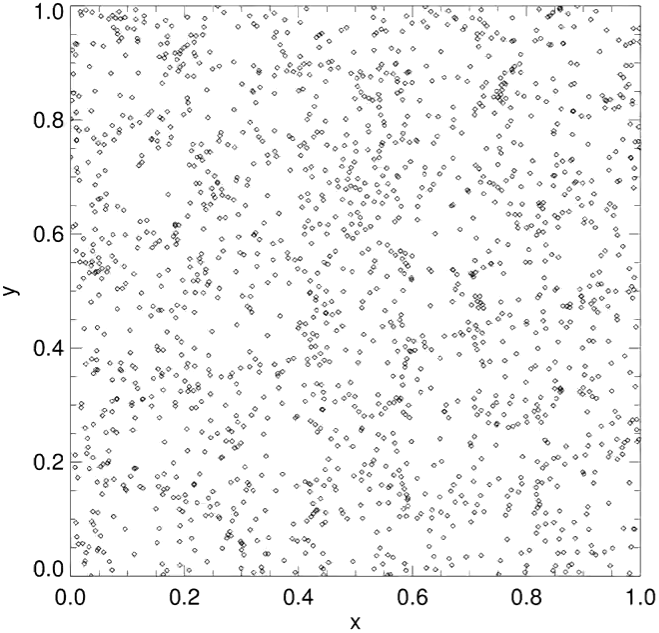
\includegraphics[width=\textwidth]{methods/no_wvt_relax_donnert.png}
  \end{subfigure}%
  ~
  \begin{subfigure}[b]{.5\textwidth}
    \centering
    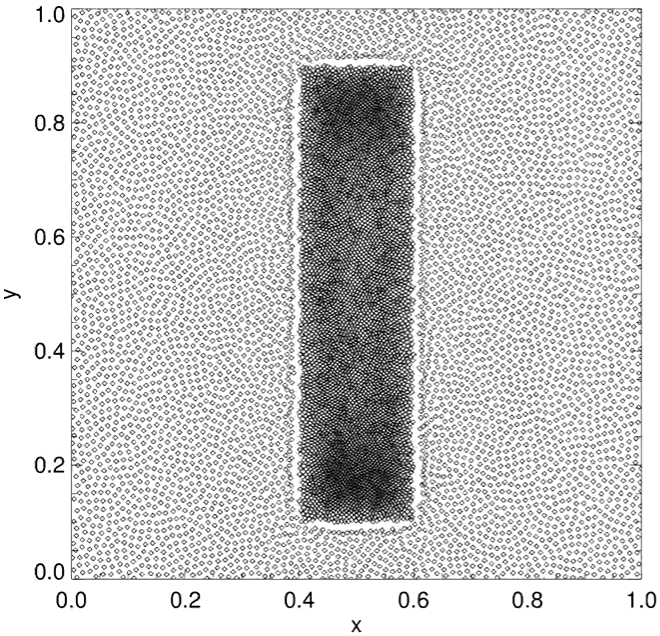
\includegraphics[width=\linewidth]{methods/yes_wvt_relax_donnert.png}
    \end{subfigure}
    \caption{\textbf{Left}: inhomogeneities in Poisson sampled particles
             prior to WVT relaxation \textbf{Right:} Post-WVT particle distribution
             showing a glass-like structure, apart from the obvious box structure 
             in the center. This feature results from introducing a density 
             discontinuity in the fluid that SPH cannot model properly.
             Stills taken from a video sent by \citet[priv. comm.]{DonnertWVT}}
    \label{fig:glass}
\end{figure}

\begin{figure}
    \centering
    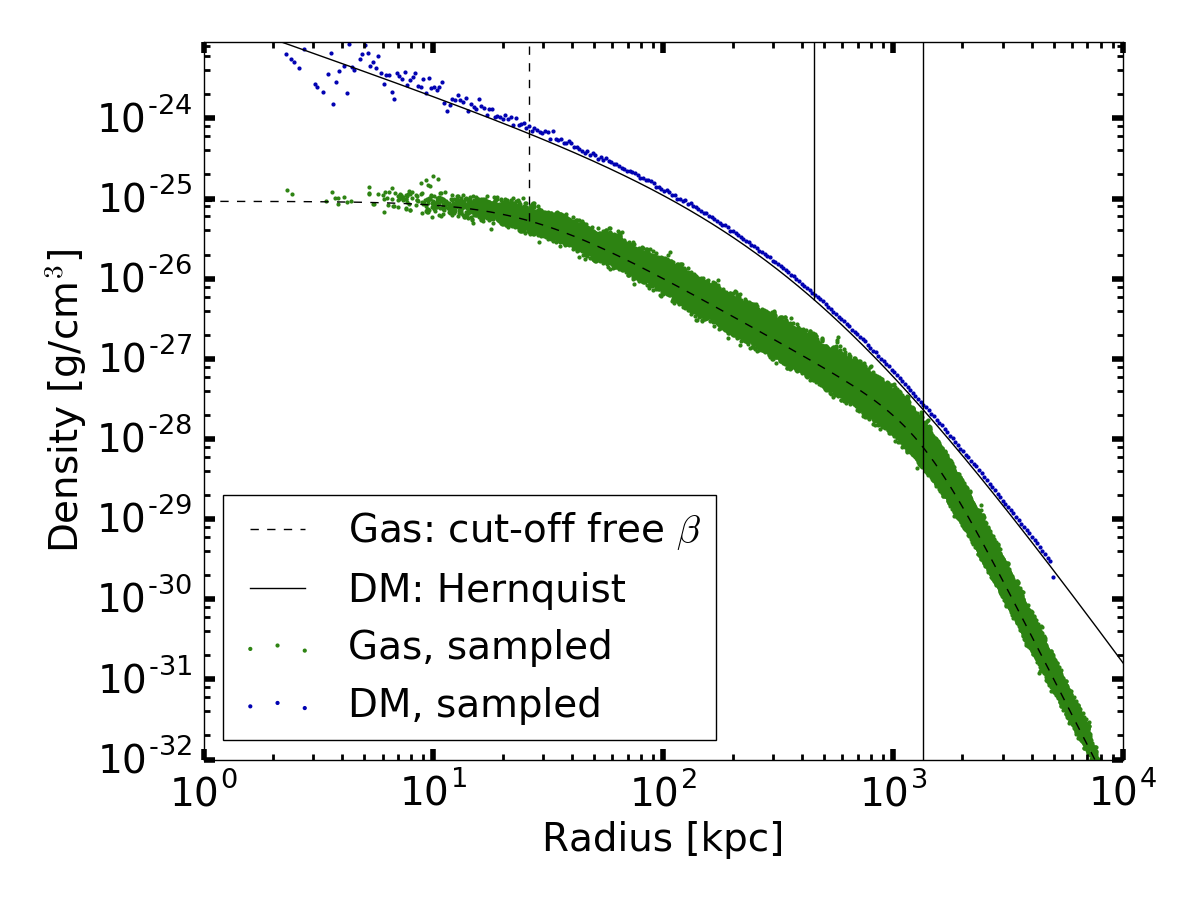
\includegraphics[width=0.78\textwidth]{methods/no_wvt_relax.png}
    \caption{Resulting dark matter (blue) and gas (green) density profiles for 
             CygA when sampling two million particles and setting the NUMITER
             variable in \code{Toycluster} to zero such that the particles are
             not relaxed using Weighted Voronoi Tesselations. The vertical lines
             that stop at the density profiles indicate the core radius $r_c$ of
             the betamodel (gas), and the Hernquist scale length $a$ (dark matter).
             The vertical line on the right indicates the virial radius $r_{200}$.}
    \label{fig:no_wvt_relax}
    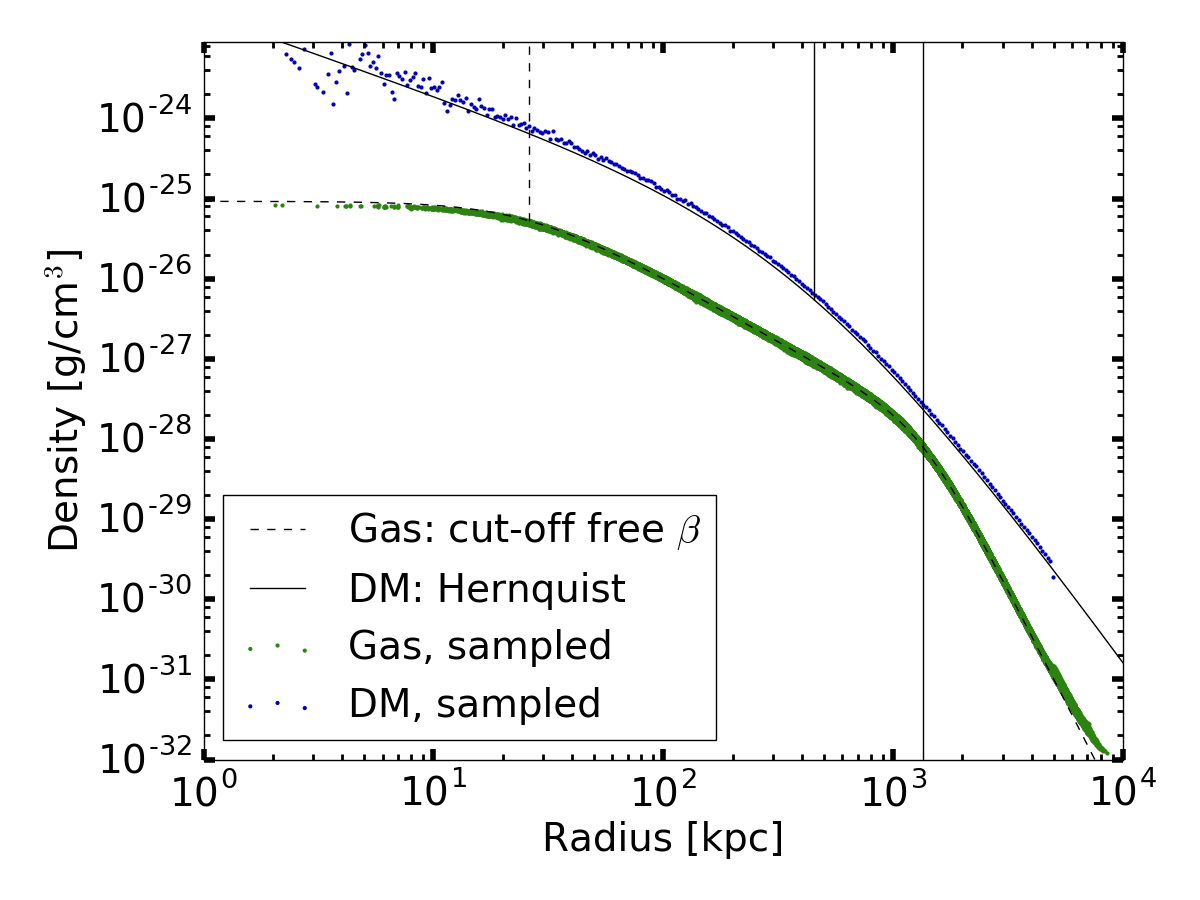
\includegraphics[width=0.78\textwidth]{methods/yes_wvt_relax.png}
    \caption{Resulting dark matter (blue) and gas (green) density profiles for
             CygA when sampling two million particles with Weighted Voronoi 
             Tesselation relaxation. The scatter around the analytically desired
             profile is significantly reduced from a $42.1$ per cent mean error 
             down to $2.6$ per cent.}
    \label{fig:yes_wvt_relax}
\end{figure}


\section*{SPH Kernel}
The initial conditions generated by \code{Toycluster} are set up to use with
a proprietary version of \code{Gadget-3} \citep{2009MNRAS.398.1678D}. We, however,
only have access to the publicly available \code{Gadget-2} \citep{2005MNRAS.364.1105S}.
The SPH kernel implemented in \code{Gadget-3} and \code{Toycluster} is the 
\citet{wendland1995piecewise, wendland2004scattered}~C6 \citep{2012MNRAS.425.1068D} 
kernel where the SPH-density is smoothed over the $295 \pm 0.01$ nearest neighbors.
The SPH-kernel in \code{Gadget-2} is the cubic B-Spline kernel \citep{1985A&A...149..135M},
where we use $50\pm2$ neighbours. The sampled initial conditions show a small
density jump within the kernel when a Wendland smoothed particle set was plugged 
in \code{Gadget-2} as the density is recalculated with the B-Spline kernel. The
small density fluctuation slowly propagates outwards, which can clearly be seen
in a video of the density profile over time. Two frames are shown in 
Figure~\ref{fig:wendland_to_bspline} where the output of \code{Toycluster} is
shown on the left, and the right panel shows the same radial density profile 
after integrating for $0.5$~Gyr with \code{Gadget-2}. The resolution scale is 
indicated by the vertical dashed green line, and the density profiles appear
to increase slightly at radii ($r \lesssim 100$) kpc. This behaviour is this
reason \code{Toycluster} is equipped with the older kernel used by \code{Gadget-2} 
in an effort to minimise the numerical consequences of swapping kernels going 
from the initial conditions to the simulation snapshots. This change can be
switched on using a compile time option.

\begin{figure}[ht]
  \centering
  %\captionsetup[subfigure]{oneside,margin={-0.25cm,0cm},width=\textwidth}
  \begin{subfigure}[b]{.5\textwidth}
    \centering
    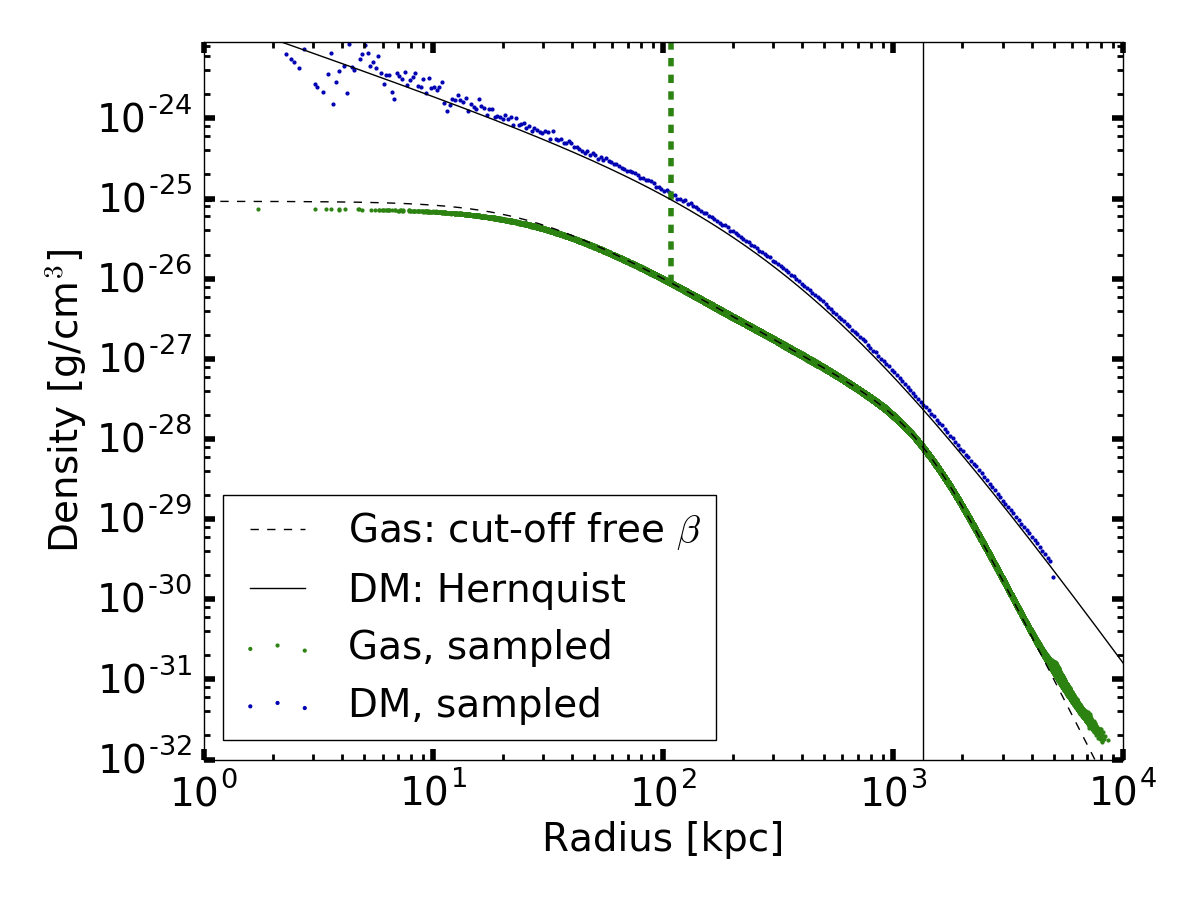
\includegraphics[width=\textwidth]{methods/wendland_to_bspline_ic.png}
    %\caption{}
    %\label{fig:wendland_to_bspline_ic}
  \end{subfigure}%
  ~
  %\captionsetup[subfigure]{oneside,margin={0.25cm,0cm}}
  \begin{subfigure}[b]{.5\textwidth}
    \centering
    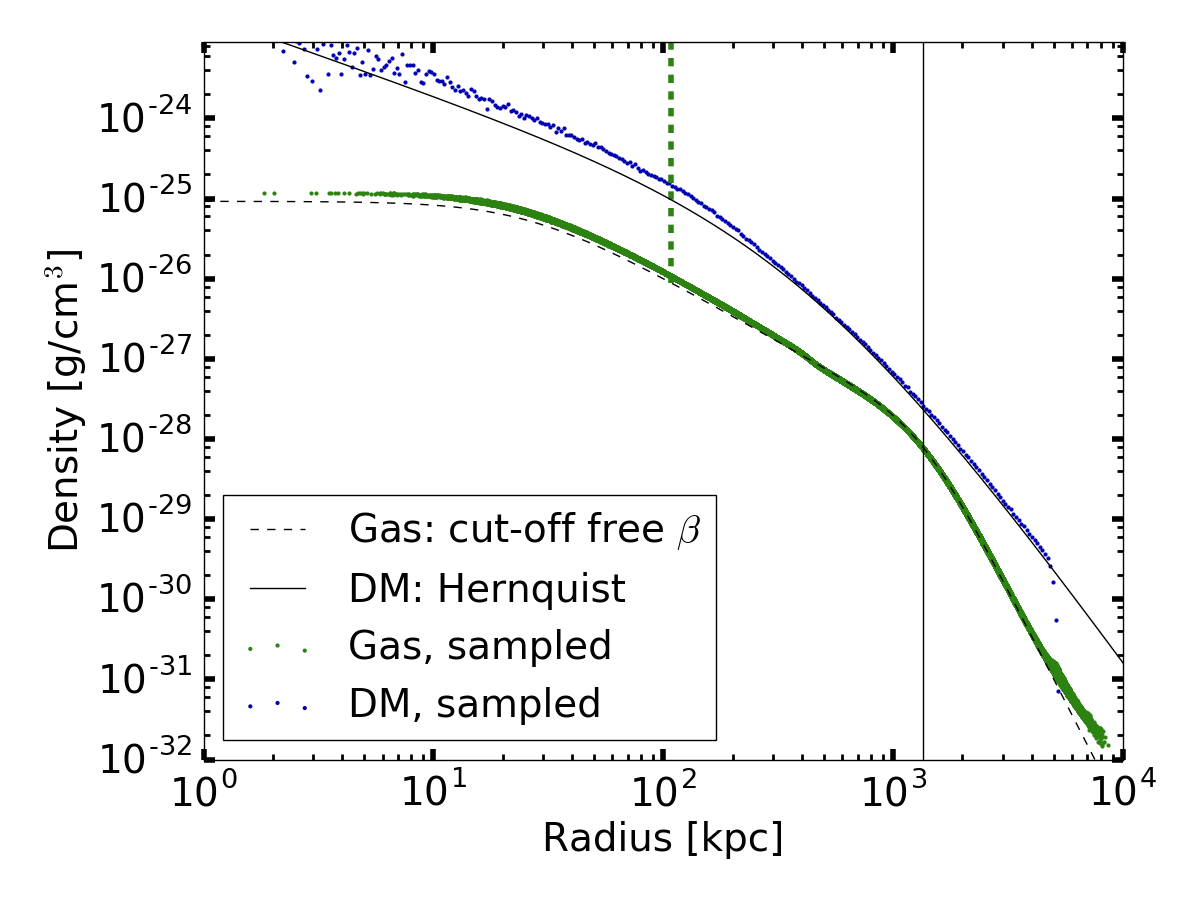
\includegraphics[width=\linewidth]{methods/wendland_to_bspline_020.png}
    %\caption{}
    %\label{fig:wendland_to_bsline_snap}
    \end{subfigure}
    \caption{\textbf{Left}: dark matter (blue) and gas (green) density profile
             of initial conditions generated for CygA with two million particles
             using the Wendland~C6 kernel. \textbf{Right:} same plot after 
             integrating for $0.5$ Gyr using the B-Spline kernel. Both profiles
             appear to 'creep up' over time inside the kernel. The dashed 
             vertical green line indicates $2h_{\text{sml}}$. Note the differences
             on the left hand side of this line ($r \lesssim 100$) kpc.}
    \label{fig:wendland_to_bspline}
\end{figure}








\section*{Further Changes}
The latest version of the code further allows to sample additional subhaloes inside
the main halo to take into account the effect of substructure. This is used 
to create extra disturbances for a study of the Sausage cluster, which is the main 
astronomical system of interest in the study by \citet{2016MNRAS.000.000D}.

Furthermore, an additional bump in the density profile at small radii can be
simulated to further increase the central density, thus, decrease the core 
temperature should one two merging haloes be a cool core cluster.

The additional substructure and the double beta cool core option can optionally 
be switched on at compile time by setting the appropriate compiler flag in the 
makefile, both of which are not used in the Cygnus study presented in this thesis.


\section{\code{Gadget-2}: Massively Parallel TreeSPH}
\label{sec:methods-gadget}

A full consideration of the numerical implementation of the combined SPH-gravity
code is beyond the scope of this thesis. We use the publicly available code 
\code{Gadget-2} \citep{2001NewA....6...79S, 2005MNRAS.364.1105S}. This code unifies
two Lagrangian particle-based methods as it combines SPH with a tree-based gravity
solver, a scheme known as TreeSPH \citep{1989ApJS...70..419H}. The  
\citet{1986Natur.324..446B}-like octree structure makes the code scale as $O(N \log N)$,
which is considerably more favourably than direct $N$-body codes.

The integrator uses the kick-drift-kick (KDK) Leapfrog scheme for time stepping.
In the purest implementation, the Leapfrog is a symplectic method. The large dynamic
range required for cosmological simulations requires individual timestepping of
particles. Should a smaller time step be required, the base-two time steps are
bitshifted such that multiple KDK's can be given to eligible particles before
a synchronisation step kicks all particles at the same time. As as result, however,
the symplectic nature of the pure Leapfrog is broken and the resulting scheme
is referred to as quasi-symplectic.


% TODO: thermodynamics in \code{Gadget-2}. Does this belong here or in theory?


\section{\code{P-Smac2}: Line-of-Sight Integrated Observables}
\label{sec:methods-psmac}
\citet{2014MNRAS.443.3564D} briefly describe a very small part of the line-of-sight 
integrating projection code \code{P-Smac2} in the appendix. The main use of this
code is that it is able to read the simulation snapshots written by \code{Toycluster}
and \code{Gadget-2}, select projection on the sky by rotating the system like
an airplane in a yaw-pitch-roll way that is parametrised by three Euler Angles,
then choose the desired physical quantity to obtain from the simulation, do the
kernel-weighted summation plus line-of-sight integration, and, finally, read
this conveniently as a Rice compressed fits data cube. These end-products of the
simulation pipeline can then be opened in SAOImage~ds9 \citep{2003ASPC..295..489J}
alongside the observed X-ray surface brightness for easy comparison between the
simulated merger and the observation.

For example, the projected X-ray surface brightness is computed between a given
energy range following \citep[][eq. 3]{1996MNRAS.283..431B}, assuming the X-rays
result from thermal Bremsstrahlung continuum emission.

\section{Pre- and post-processing}
\label{sec:python}

Numerous \code{Python} and \code{bash} scripts have been written by the author
to standardize the calling sequence of the simulation pipeline. This way we
automatically organise the simulation output in a systematic way that allows us
to easily keep track of the models we ran. The countless options would otherwise 
make it rather difficult to keep track of differences in the parameter space
and the rather confusing forrest of both compile- and runtime options. At times
of writing the total code base contains $8524$ self-written lines of \code{Python},
and $2680$ self-written lines of \code{bash}. The simulation pipeline relies
on the \code{OpenMP} parallel c99 code \code{Toycluster} with $6131$ code lines,
the \code{MPI} parallel c99 \code{Gadget-2} consisting of $17804$ lines, and 
\code{P-Smac2} with $7539$ lines of hybrid \code{OpenMP}/\code{MPI} c99. Naturally, 
this leads to a three-fold directory structure to store the simulations. 
Every simulation run given a timestamp folder containing an initial conditions, 
simulation, and analysis subfolders. We compile all three programs for every 
simulation run, move it to the appropriate location, and copy all parameter- and
Makefiles used as part of the output. Finally, any output written to stdout and 
stderr is captured and piped to a log file in the relevant directory.

Post-processing is done using the \code{amuse} framework
\citep{2009NewA...14..369P, 2013CoPhC.183..456P, 2013A&A...557A..84P}. For example,
the binary \code{Fortran 77} output files containing the particles are parsed and stored 
in the \code{amuse} datamodel. In addition, the \code{amuse} unit module is used 
to handle physical unit conversions, and \code{matplotlib} is used to generate 
plots. Relevant \code{Python} packages are imported when needed. As of yet, all
self-written code lives in a private GitHub repository, but should \code{Toycluster} 
become publicly available we intent to also open up our repository.

\SubfileBibliography
\end{document}
